\documentclass[11pt,letterpaper]{article}
\usepackage{fullpage}
\usepackage[top=0.5in, bottom=1.5in, left=1in, right=1in]{geometry}
\usepackage{amsmath,amsthm,amsfonts,amssymb,amscd}
\usepackage{lastpage}
\usepackage{enumerate}
\usepackage{enumitem}
\usepackage{fancyhdr}
\usepackage{graphicx}
\usepackage{listings}
\usepackage{hyperref}
\usepackage{booktabs}
\usepackage{cancel}
\usepackage{physics}
\usepackage{caption,cleveref,colortbl,csquotes,datatool,helvet,mathpazo,multirow,listings,pgfplots,xcolor}

\hypersetup{%
  colorlinks=true,
  linkcolor=blue,
  linkbordercolor={0 0 1}
}

\setlength{\parindent}{0.0in}
\setlength{\parskip}{0.05in}
\setlength{\footnotesep}{1.2\baselineskip}


% edit these
\newcommand\course{AST222H}
\newcommand\Title{Problem Set 5}
\newcommand\Name{Jeff Shen} 
\newcommand\Id{1004911526} 
\newcommand\Date{3 Apr 2020}

\pagestyle{fancyplain}
\headheight 35pt
\lhead{\Name}
\lhead{\Name\\\Id}
\chead{\LARGE \Title}
\rhead{\course \\ \Date}
\lfoot{}
\cfoot{}
\rfoot{\small\thepage}
\pgfplotsset{compat=1.16}
\headsep 1.2em

\begin{document}

\section*{Problem 1}

Using the distance modulus formula, this distance is (ignoring extinction)
\begin{align*}
    d = 10^{(m-M+5)/5} = 10^{(25+19.5+5)/5} = 7.94~{\rm Gpc}.
\end{align*}

\section*{Problem 2}
Density for matter is given by $\rho_{m,\,0} = \Omega_{m,\,0}(1+z)^3$, and for radiation by $\rho_{r,\,0} = \Omega_{r,\,0}(1+z)^4$. Equate the two and solve for $z$:
\begin{alignat*}{2}
    &&\rho_{m,\,0} &= \rho_{r,\,0} \\
    \implies&&\Omega_{m,\,0}(1+z)^3 &= \Omega_{r,\,0}(1+z)^4 \\
    \implies&&z &= \frac{\Omega_{m,\,0}}{\Omega_{r,\,0}} - 1 = \frac{0.317}{10^{-4}} - 1 = 3169.
\end{alignat*}

\section*{Problem 3}

The radius of the sphere of influence of the black hole is 
\begin{align*}
    r = \frac{GM}{\sigma^2} = \frac{6.67\times 10^{-11}~{\rm m^3\,kg^{-1}}\times 2\times 10^{9}~{\rm M_\odot}}{4\times 10^{5}~{\rm m\,s^{-1}}} = 1.66\times 10^{18}~{\rm m}.
\end{align*}

Given that the distance to M87 is $53.5~{\rm Mly} = 5.06\times 10^{23}~{\rm m}$, the angular radius is 
\begin{align*}
    \theta \simeq \tan{\theta} = \frac{r}{d} = \frac{1.66\times 10^{18}~{\rm m}}{5.06\times 10^{23}~{\rm m}} = 3.28\times 10^{-6}~{\rm rad} = 0.67~{\rm arcsec}.
\end{align*}

Whether this is observable without adaptive optics probably depends on the location of the ground-based telescope and the atmospheric conditions. The Internet\footnote{Racine, R. 1989, Publications of the Astronomical Society of the Pacific, 101, 436.} and the lecture slides from week 1 say that seeing of 0.5" can be achieved in locations such as Mauna Kea.  

\section*{Problem 4}

The parallax formula is 
\begin{alignat*}{2}
    &&\theta \simeq \tan{\theta} &= \frac{r}{d} \\
    \implies&& d &= \frac{r}{\theta},
\end{alignat*}
where $d$ is the distance we want, $\theta$ is the parallax angle, and $r$ is the distance from Gaia to the Sun. Gaia is at the Earth-Sun L2 Lagrangian point, which has a radius of orbit of approximately $1.01~{\rm au}$. Plugging these values in, we find that $d$ is 
\begin{align*}
    d = \frac{1.01~{\rm au}}{0.05~{\rm arcsec}} = 20.22~{\rm pc}.
\end{align*}
At this distance, 

\newpage

\section*{Problem 5}

\begin{figure*}[!htbp]
    \centering
    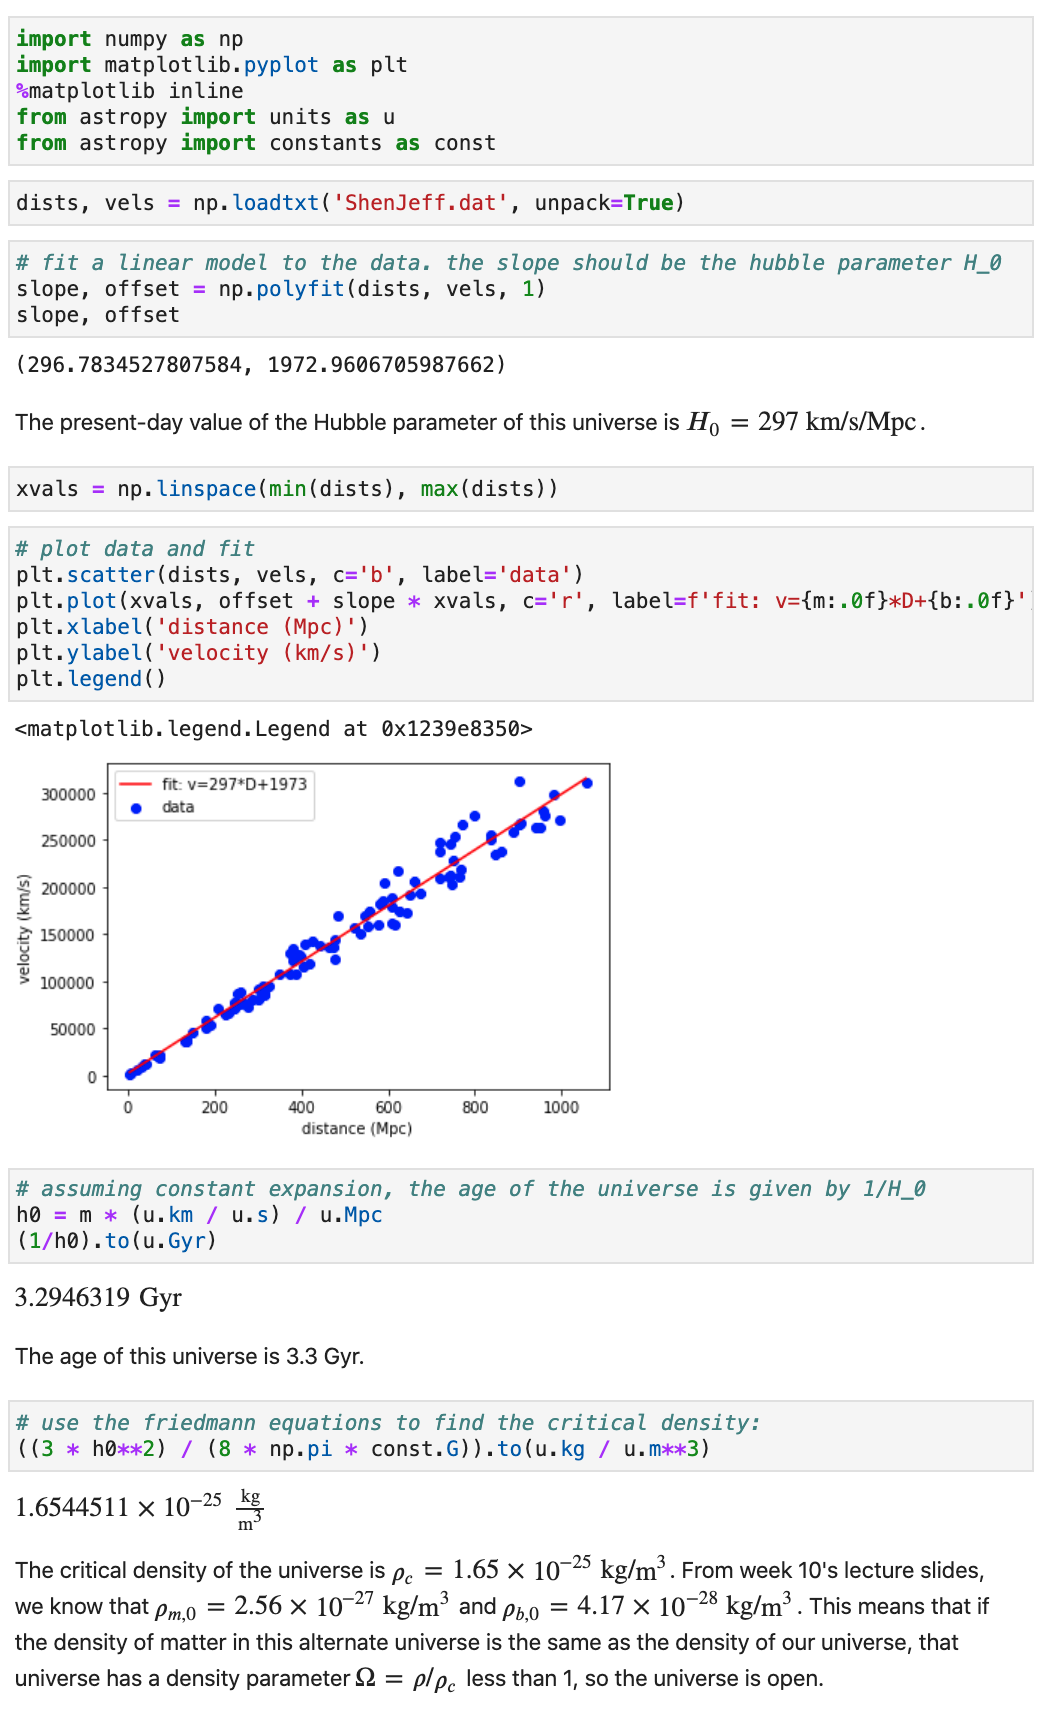
\includegraphics[width=0.78\linewidth]{q5.png}
\end{figure*}

\newpage

\section*{Problem 6}
\begin{enumerate}[label=(\roman*)]
    \item C\&O Eq. 29.10:
        \begin{align*}
            \left[\left(\frac{1}{R}\frac{dR}{dt}\right)^2 - \frac{8}{3}\pi G\rho\right]R^2 = -kc^2.
        \end{align*}
        Multiplying this by $R$, we get 
        \begin{align*}
            \left(\frac{dR}{dt}\right)^2 R - \frac{8}{3}\pi G\rho R^3 = -kc^2R 
        \end{align*}
        Taking the time derivative and applying the product and chain rules to the first term, we get 
        \begin{align*}
            2\frac{dR}{dt}\frac{d^2R}{dt}R + \left(\frac{dR}{dt}\right)^3 - \frac{8}{3}\pi G \frac{d}{dt}(\rho R^3) = \frac{d}{dt}(-kc^2R).
        \end{align*}
        We use C\&O Eq. 29.50 to replace the third term on the left side, then expand the derivative using the chain rule and cancel out a $dR/dt$ term:
        \begin{alignat*}{2}
            &&2\frac{dR}{dt}\frac{d^2R}{dt^2}R + \left(\frac{dR}{dt}\right)^3 + \frac{8}{3}\pi G\frac{P}{c^2}\frac{d(R^3)}{dt} &= -kc^2\frac{dR}{dt} \\
            \implies&&2\frac{dR}{dt}\frac{d^2R}{dt^2}R + \left(\frac{dR}{dt}\right)^3 + \frac{8}{3}\pi G\frac{P}{c^2}3R^2\frac{dR}{dt} &= -kc^2\frac{dR}{dt} \\
            \implies&&2\frac{d^2R}{dt^2}R + \left(\frac{dR}{dt}\right)^2 + 8\pi G\frac{P}{c^2}R^2 &= -kc^2.
        \end{alignat*}
        We can use Eq. 29.10 again to replace the $-kc^2$ term on the right side: 
        \begin{align*}
            2\frac{d^2R}{dt^2}R + \left(\frac{dR}{dt}\right)^2 + 8\pi G\frac{P}{c^2}R^2 &= \left(\frac{dR}{dt}\right)^2 - \frac{8}{3}\pi G\rho R^2.
        \end{align*}
        Cancelling terms and rearranging, we get 
        \begin{align*}
            2\frac{d^2R}{dt^2}R = -8\pi GR^2(\frac{\rho}{3} + \frac{P}{c^2}).
        \end{align*}
        Dividing both sides by $2R$ and then factoring out $1/3$ from the right side, we arrive at C\&O Eq. 29.51:
        \begin{align*}
            \frac{d^2R}{dt^2} = -\frac{4}{3}\pi GR(\rho + \frac{3P}{c^2}).
        \end{align*}

    \item From C\&O Eq. 29.8, we know that 
        \begin{align}
            HR = \frac{dR}{dt},
        \end{align}
        and by (a rearrangement of) the definition of the density parameter $\Omega$, we know that 
        \begin{align}
            H^2 = \frac{8\pi G\rho}{3\Omega}.
        \end{align}
        Using Eq. 1 and Eq. 2 above to replace the denominator of the expression for the deceleration parameter, and the acceleration equation to replace the numerator, we can rewrite the deceleration parameter as 
        \begin{equation*}
        \setlength{\jot}{10pt}
            \begin{align*}
                q &= -\frac{R\frac{d^2R}{dt^2}}{(\frac{dR}{dt})^2} \\
                &= -\frac{R\frac{d^2R}{dt^2}}{H^2R^2} \\
                &= -\frac{\frac{d^2R}{dt^2}}{H^2R} \\
                &= -\frac{-\frac{4}{3}\pi GR(\rho + \frac{3P}{c^2})}{\frac{8\pi G\rho}{3\Omega}R} \\
                &= \frac{\rho + \frac{3P}{c^2}}{\frac{2\rho}{\Omega}} \\
                &= \frac{\frac{\rho c^2 + 3P}{c^2}}{\frac{2\rho}{\Omega}} \\
                &= \frac{(\rho c^2 + 3P)\Omega}{2\rho c^2}.
            \end{align*}
        \end{equation*}
        Using the equation of state $P=\omega \rho c^2$ to replace the $P$ in the above expression, we get 
        \begin{equation*}
        \setlength{\jot}{10pt}
            \begin{align*}
                q &= \frac{(\rho c^2 + 3\omega \rho c^2)\Omega}{2\rho c^2} \\
                &= \frac{\Omega\rho c^2(1+3\omega)}{2\rho c^2} \\
                &= \frac{\Omega}{2}(1+3\omega). 
            \end{align*}
        \end{equation*}

    \item We begin with multiplying the acceleration by $R^2$ to get 
        \begin{align*}
            \frac{d^2R}{dt^2}R^2 = -\frac{4}{3}\pi GR^3(\rho + \frac{3P}{c^2}).
        \end{align*}
        Taking the time derivative and applying the product rule to the left side and the chain rule to both sides, we get 
        \begin{align*}
            \frac{d^3R}{dt^3}R^2 + \frac{d^2R}{dt^2}2R\frac{dR}{dt} = -\frac{4}{3}\pi G3R^2\frac{dR}{dt}(\rho + \frac{3P}{c^2}).
        \end{align*}
        We can cancel out an $R$ term, move the second term from the left to the right side, then multiply both sides of the equation by $R^2/(dR/dt)^3$ to get the expression for jerk on the left:
        \begin{align*}
            j(t) = \frac{R^2\frac{d^3R}{dt^3}}{(\frac{dR}{dt})^3} = -4\pi GR^3\left(\frac{dR}{dt}\right)^{-2}\left(\rho + \frac{3P}{c^2} + 2\frac{d^2R}{dt^2}\frac{1}{4\pi GR}\right).
        \end{align*}
        Using Eq. 1 from Q6(ii), we can introduce an $H$ term into the right side:
        \begin{align*}
            j(t) = -\frac{4\pi GR}{H^2}\left(\rho + \frac{3P}{c^2} + \frac{\frac{d^2R}{dt^2}}{2\pi GR}\right).
        \end{align*}
        We can use the equation of state to replace the first two terms in the parentheses, and the acceleration equation to replace the numerator in the last term: 
        \begin{align*}
            j(t) = -\frac{4\pi GR}{H^2}\left(\rho(1+3\omega) - \frac{\frac{4}{3}\pi GR(\rho + \frac{3P}{c^2})}{2\pi GR}\right).
        \end{align*}
        After cancelling terms, we can again use the equation of state to rewrite the last term:
        \begin{align*}
            j(t) &= -\frac{4\pi GR}{H^2}\left(\rho(1+3\omega) - \frac{2}{3}(\rho(1+3\omega))\right) = -\frac{\frac{4}{3}\pi GR\rho(1+3\omega)}{H^2}.
        \end{align*}
        Using Eq. 2 from Q6(ii), we replace the $H^2$ term and arrive at an expression for $j$ in terms of $\Omega$ and $\omega$:
        \begin{align*}
            j(t) = -\frac{\frac{4}{3}\pi GR\rho(1+3\omega)}{\frac{8\pi GR\rho}{3\Omega}} = -\frac{R\Omega}{2}(1+3\omega).
        \end{align*}
        For matter, with $\omega=0$, we get 
        \begin{align*}
            j(t) = -\frac{R\Omega}{2}(1+0) = -\frac{R\Omega}{2},
        \end{align*}
        and for dark energy, with $\omega=-1$, we get 
        \begin{align*}
            j(t) = -\frac{R\Omega}{2}(1-3) = R\Omega.
        \end{align*}

\end{enumerate}



\end{document}
